\section{N8N хэрэгжүүлэлт}
% \subsection{N8N ажлын урсгал}
Үндсэн ажлын урсгалд гол үйлдэл болон зангилаанууд угсрагдсан. Хэрэглэгчдэд зориулсан хариултыг энэ урсгал ажиллана.
\begin{figure}[H]
    \centering
    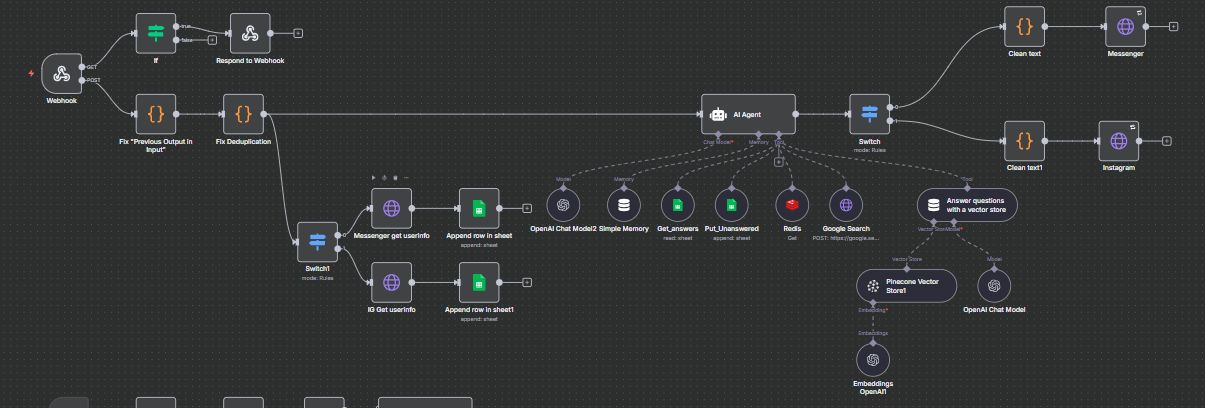
\includegraphics[scale=0.5]{assets/Screenshot 2025-09-04 154908.png}
    \caption{Үндсэн цөм ажлын урсгал}
    \label{fig:main_workflow}
\end{figure}
Google драйв дээр хадгалсан компанийн мэдээлэл бүхий файлуудыг татаж аван pinecone vector store зангилаа ашиглан chunk-уудад хуваан тоон хэлбэр лүү задлан хадгална.
\begin{figure}[H]
    \centering
    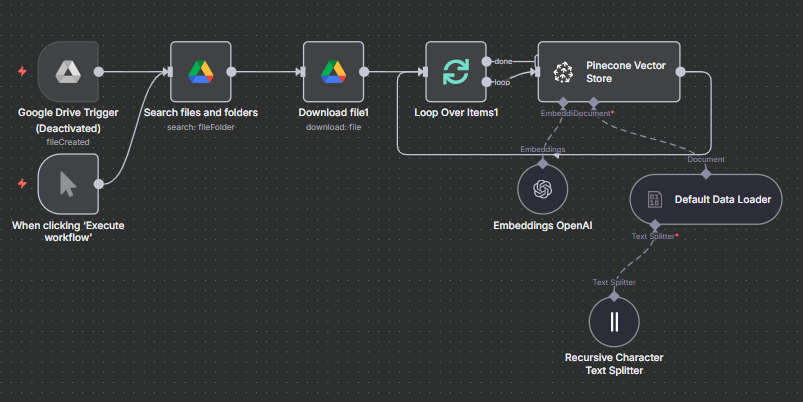
\includegraphics[scale=0.7]{assets/Screenshot 2025-09-04 154942.png}
    \caption{Pinecone векторт өгөгдөл оруулах}
    \label{fig:pinecone_input}
\end{figure}
Тодорхой цагаар буюу МХБ-ийн арилжааны цагийн үеэр 5 минут тутам ажиллан өсөлттэй, бууралттай хувьцааны мэдээллийг БиДиСек компанийн redis VPS сервер дээр хадгална.
\begin{figure}[H]
    \centering
    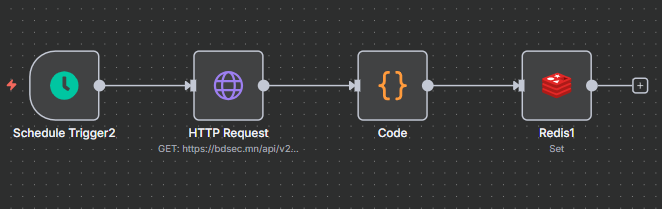
\includegraphics[scale=0.7]{assets/Screenshot 2025-09-04 154951.png}
    \caption{Redis дээр өсөлттэй бууралттай хувьцааны мэдээлэл хадгалах хуваарьт ажлын урсгал}
    \label{fig:redis_scheduled}
\end{figure}
7 хоногийн ажлын өдрүүдэд арилжааны цаг болон 10:00-аас 13:00 цаг хүртэл 5 минут тутам ажиллахаар тохируулсан.
\begin{figure}[H]
    \centering
    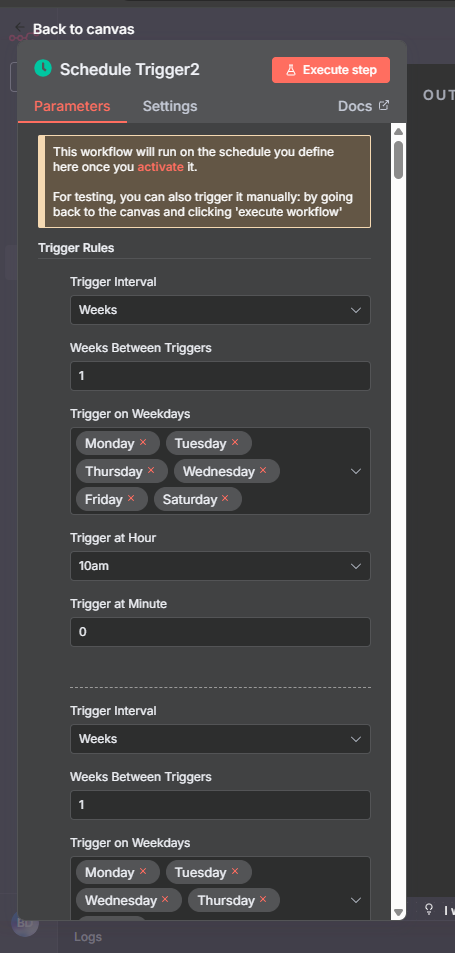
\includegraphics[scale=0.7]{assets/Screenshot 2025-09-04 155020.png}
    \caption{Хуваариар ажилладаг ажлын урсгал}
    \label{fig:scheduled_workflow}
\end{figure}

БиДиСек компанийн API-аас авсан бүх хувьцааны мэдээллээс хамгийн өсөлттэй, бууралттай хувьцаануудыг ялгаж авах үүрэгтэй код.
\textbf{Өсөлттэй бууралттай хувьцааны мэдээллийг форматжуулах код}

\begin{lstlisting}[language=Java, caption=Хувьцааны мэдээлэл харуулах, frame=single]
/**
 * Clean Top Gainers / Losers (no debug, no prefix).
 *
 * Rules:
 *  - Volume > 0
 *  - Change != 0
 *  - Gainers: change > 0 (desc)
 *  - Losers : change < 0 (asc)
 *  - Symbol: '-' хүртэлх хэсгийн үсгүүдийг том үсгээр
 *  - Output fields per line: Symbol, PreviousClose, Changes
 */

const CONFIG = {
  TOP_N: 10,
  TIMEZONE: 'Asia/Ulaanbaatar',
  LOCALE: 'mn-MN',
  DECIMALS_PRICE: 4,
  DECIMALS_CHANGE: 4,
};

function normalizeMinus(str) {
  if (typeof str !== 'string') return str;
  return str.replace(/[\u2212\u2012\u2013\u2014]/g, '-');
}

function toNumber(val) {
  if (val === null || val === undefined) return 0;
  if (typeof val === 'number') return Number.isFinite(val) ? val : 0;
  let s = normalizeMinus(String(val).trim());
  s = s.replace(/[%\s,]/g, '');
  const m = s.match(/[+\-]?\d+(\.\d+)?/);
  if (!m) return 0;
  const n = parseFloat(m[0]);
  return Number.isFinite(n) ? n : 0;
}

function simplifySymbol(sym) {
  if (!sym) return '';
  let base = String(sym).trim().split('-')[0];
  const letters = base.match(/[A-Za-z]+/g);
  return (letters ? letters.join('') : base).toUpperCase();
}

function pickFirst(obj, names) {
  for (const n of names) {
    if (obj[n] !== undefined && obj[n] !== null && obj[n] !== '') return obj[n];
  }
  return undefined;
}

function fmtPrice(n) {
  return Number.isFinite(n) ? Number(n.toFixed(CONFIG.DECIMALS_PRICE)) : n;
}
function fmtChange(n) {
  if (!Number.isFinite(n)) return n;
  const v = Number(n.toFixed(CONFIG.DECIMALS_CHANGE));
  return v > 0 ? `+${v}` : `${v}`;
}

// 1) Input массив
let data = $input.first()?.json?.data ??
           $json.data ?? $json.body ?? $json.results ?? $json;

if (typeof data === 'string') {
  try { data = JSON.parse(data); } catch { data = []; }
}
if (!Array.isArray(data)) data = [];

// 2) Цэвэрлэх
const rows = data.map(r => {
  const symbolRaw = pickFirst(r, ['Symbol','symbol','s','Ticker','ticker']);
  const symbol = simplifySymbol(symbolRaw);

  const prevCloseRaw = pickFirst(r, ['PreviousClose','PrevClose','previousClose','c','PClose','pclose']);
  const lastRaw      = pickFirst(r, ['Last','last','LastPrice','Close','close','Price','price','l']);
  const volumeRaw    = pickFirst(r, ['Volume','volume','v','Vol','vol','TradeVolume','tradeVolume']);
  const changeRaw    = pickFirst(r, ['Changes','Change','change','changePercent','ChangePercent','pctChange','PctChange','d']);

  const previousClose = toNumber(prevCloseRaw);
  const lastPrice     = toNumber(lastRaw);
  let changeVal       = toNumber(changeRaw);

  if ((changeRaw === undefined || changeVal === 0) && previousClose && lastPrice && lastPrice !== previousClose) {
    changeVal = lastPrice - previousClose;
  }

  const volume = toNumber(volumeRaw);

  return {
    symbol,
    previousClose,
    lastPrice,
    changeVal,
    volume,
  };
}).filter(r => r.symbol);

// 3) Шүүлт (Volume > 0, Change != 0)
const tradable = rows.filter(r => r.volume > 0 && r.changeVal !== 0);

// 4) Gainers / Losers
const gainers = tradable
  .filter(r => r.changeVal > 0)
  .sort((a,b) => b.changeVal - a.changeVal)
  .slice(0, CONFIG.TOP_N);

const losers = tradable
  .filter(r => r.changeVal < 0)
  .sort((a,b) => a.changeVal - b.changeVal)
  .slice(0, CONFIG.TOP_N);

// 5) Format list
function formatList(title, arr) {
  if (!arr.length) return `${title}:\n(Мэдээлэл алга)\n`;
  return `${title}:\n` + arr.map((o,i) =>
    `${i+1}. ${o.symbol} | PreviousClose: ${fmtPrice(o.previousClose)} | Changes: ${fmtChange(o.changeVal)}`
  ).join('\n') + '\n';
}

// 6) Timestamp
const ts = new Intl.DateTimeFormat(CONFIG.LOCALE, {
  timeZone: CONFIG.TIMEZONE,
  year: 'numeric', month: '2-digit', day: '2-digit',
  hour: '2-digit', minute: '2-digit', hour12: false
}).format(new Date());

// 7) Output
const output =
`${ts}-ийн байдлаар
${formatList('Топ өсөлттэй хувьцаа', gainers)}
${formatList('Топ уналттай хувьцаа', losers)}
Анхаар: `;

return { response: String(output) };
\end{lstlisting}
Ажлын урсгал амжилттай ажилласан нь харагдаж байна.
\begin{figure}[H]
    \centering
    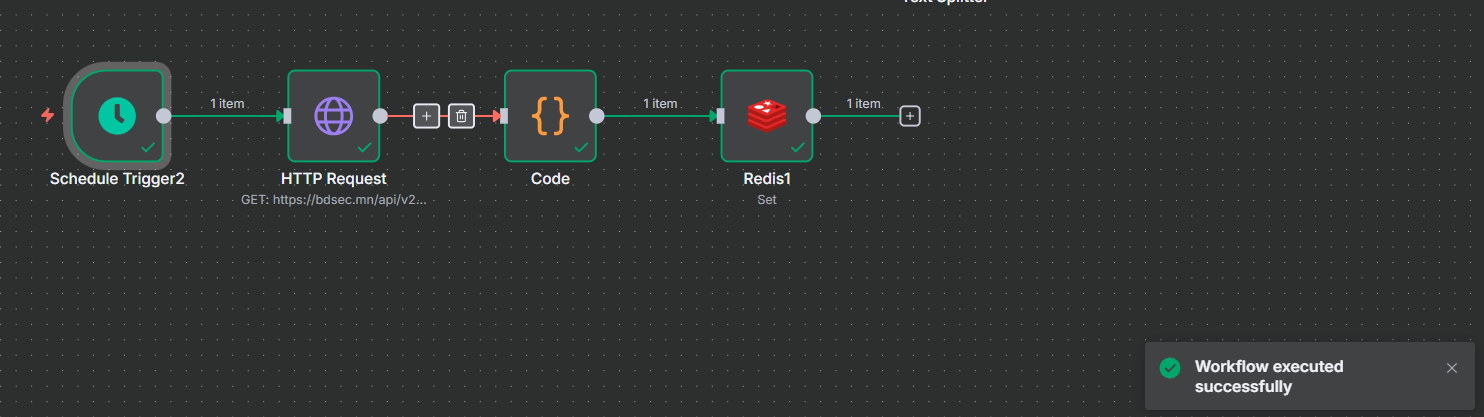
\includegraphics[scale=0.35]{assets/Screenshot 2025-09-04 155307.png}
    \caption{Redis-д хувьцааны мэдээллийг хадгалсан}
    \label{fig:redis_saved}
\end{figure}

\textbf{Үр дүн:}
\begin{figure}[H]
    \centering
    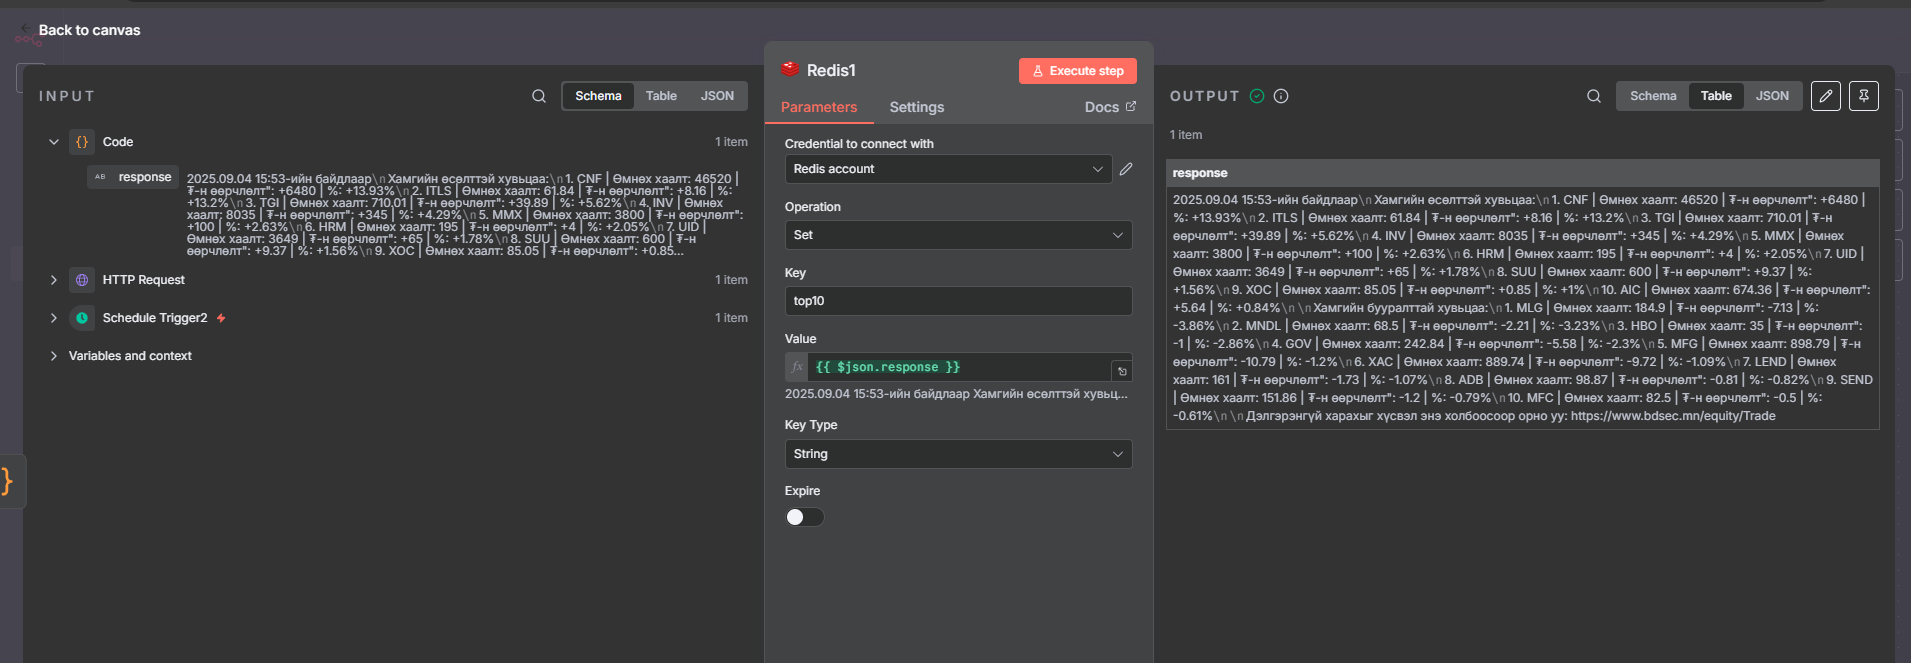
\includegraphics[scale=0.35]{assets/Screenshot 2025-09-04 155326.png}
    \caption{Хувьцааны мэдээллийн үр дүн}
    \label{fig:stock_result}
\end{figure}

Үндсэн ажлын урсгалын хиймэл оюуны зангилааны хэсэг. Үүнд openai хиймэл оюуны модел, энгийн санах ой, google sheet 2 хэрэгсэл, redis хэрэгсэл, SerperAPI хэрэгсэл болон асуултад хариулах зориулалттай pinecone vector хэрэгслүүдийг ашигласан. Openai модел нь асуултад хариулт боловсруулах гол тархины үүрэг гүйцэтгэнэ. Энгийн санах ой нь хэрэглэгчийн өмнөх чатуудыг хадгалан, түүнийгээ ашиглан хариултад хэрэглэн боловсруулалт хийдэг. Get answer(Google sheet)хэрэгсэл нь өмнө хариулж чадаагүй асуултуудад брокер хариулсан хариултыг авна. Put answer(Google sheet) хэрэгсэл нь хиймэл оюунт агент хариулж чадаагүй асуултуудаа тэмдэглэхэд хэрэглэнэ. Redis хэрэгсэл нь стринг хэлбэрээр хадгалсан датаг татаж авах зориулагдсан. SerperAPI нь хэрэглэгчийн асуултыг google-ээс хайхад хэрэглэнэ. 
\begin{figure}[H]
    \centering
    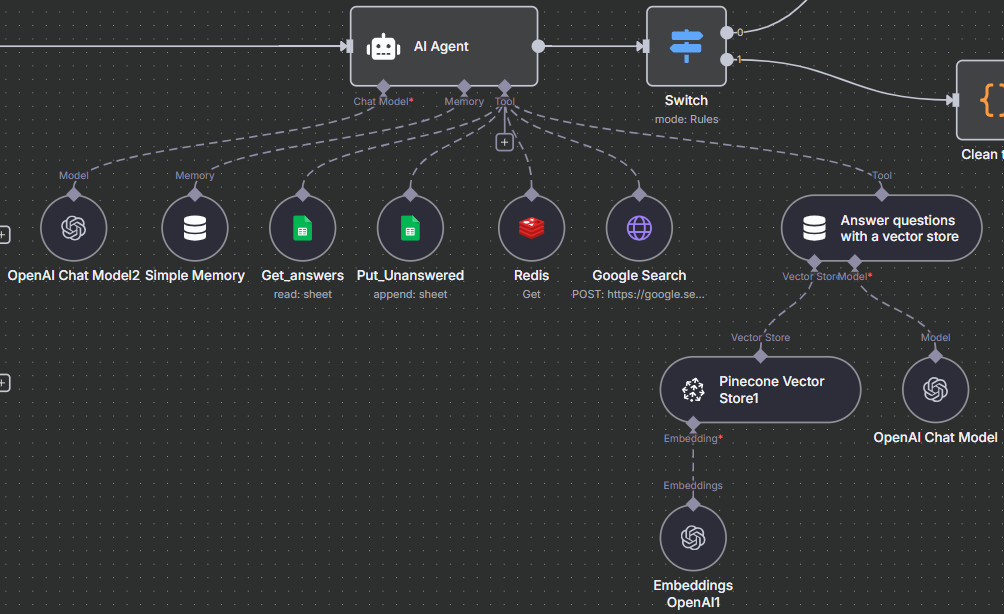
\includegraphics[scale=0.5]{assets/Screenshot 2025-09-04 155046.png}
    \caption{AI agent зангилаа болон түүний хэрэгслүүд}
    \label{fig:n8n4}
\end{figure}

\begin{figure}[H]
    \centering
    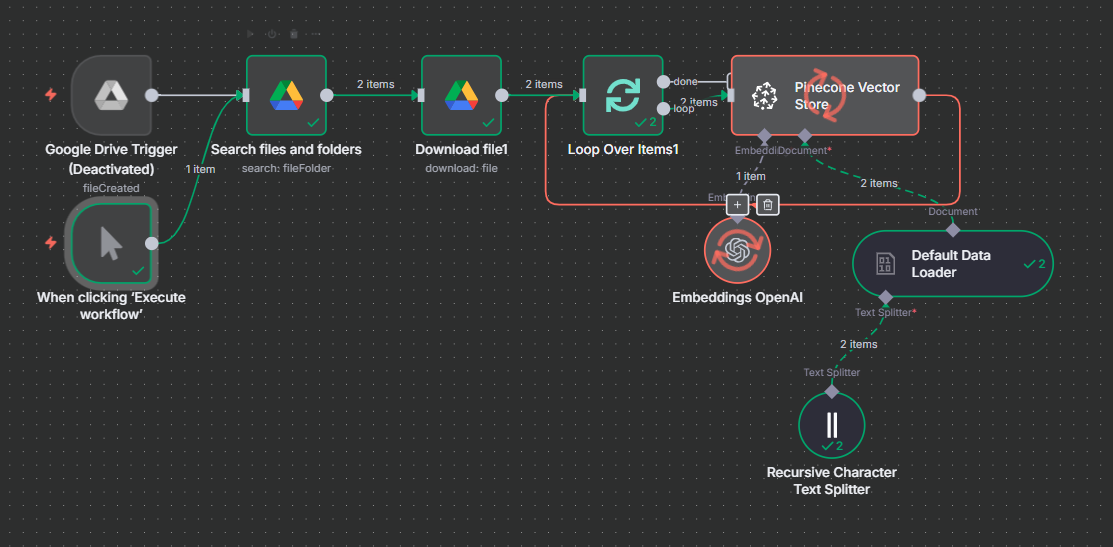
\includegraphics[scale=0.5]{assets/Screenshot 2025-09-04 155353.png}
    \caption{Вектор мэдээллийн санд дата хадгалах ажиллагааний зураг}
    \label{fig:n8n5}
\end{figure}
Ажлын урсгал амжилттай болсон нь харагдаж байна.
\begin{figure}[H]
    \centering
    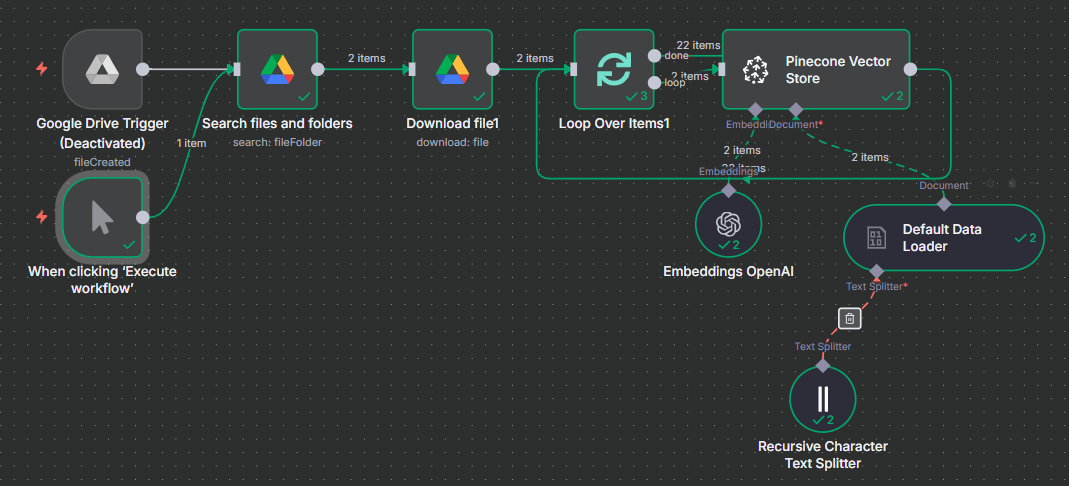
\includegraphics[scale=0.5]{assets/Screenshot 2025-09-04 155400.png}
    \caption{Вектор мэдээллийн санд дата хадгалах}
    \label{fig:n8n6}
\end{figure}

\textbf{Ажиллуулсны дараах үр дүн}

\begin{figure}[H]
    \centering
    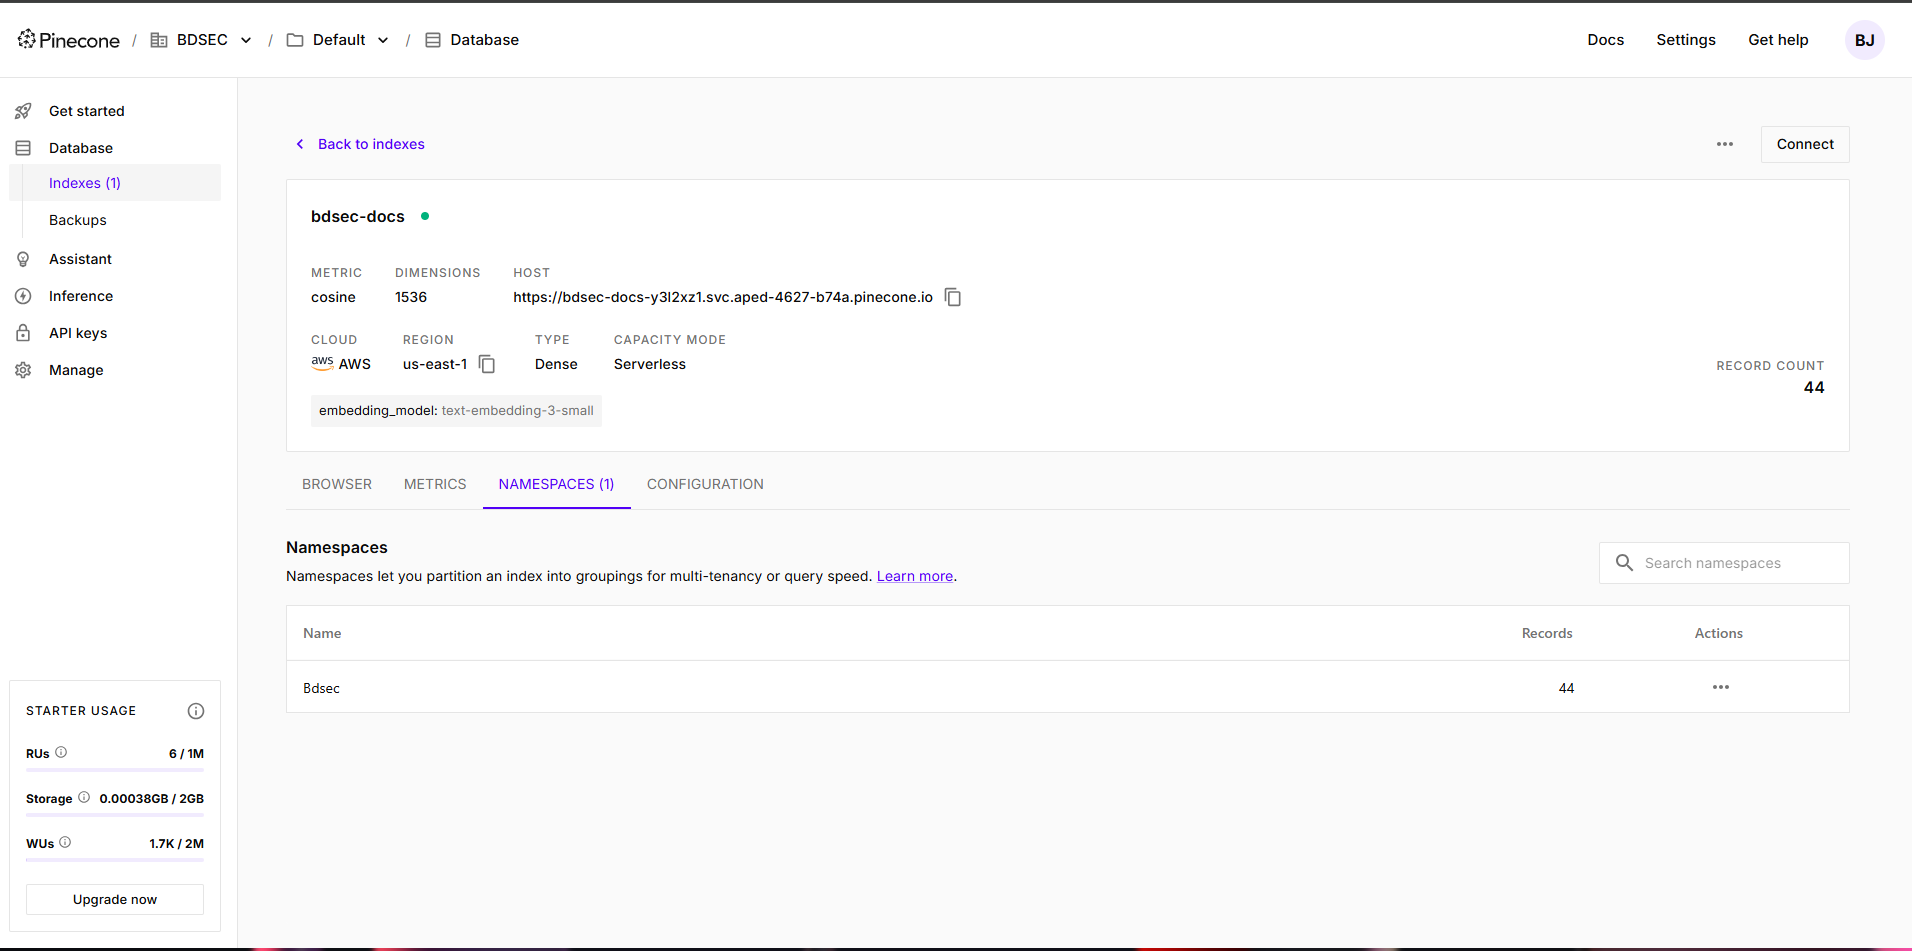
\includegraphics[scale=0.3]{assets/Screenshot 2025-09-04 163355.png}
    \caption{Pinecone вектор мэдээллийн сан}
    \label{fig:pinecone_vector_store}
\end{figure}
Бичлэг болгонд хуудас болон аль мөрнөөс аль мөрний текст агуулагдаж байгаа нь харагдаж байна.
Өгөгдөл тоон хэлбэрээр хадгалагдсан байдал:
\begin{figure}[H]
    \centering
    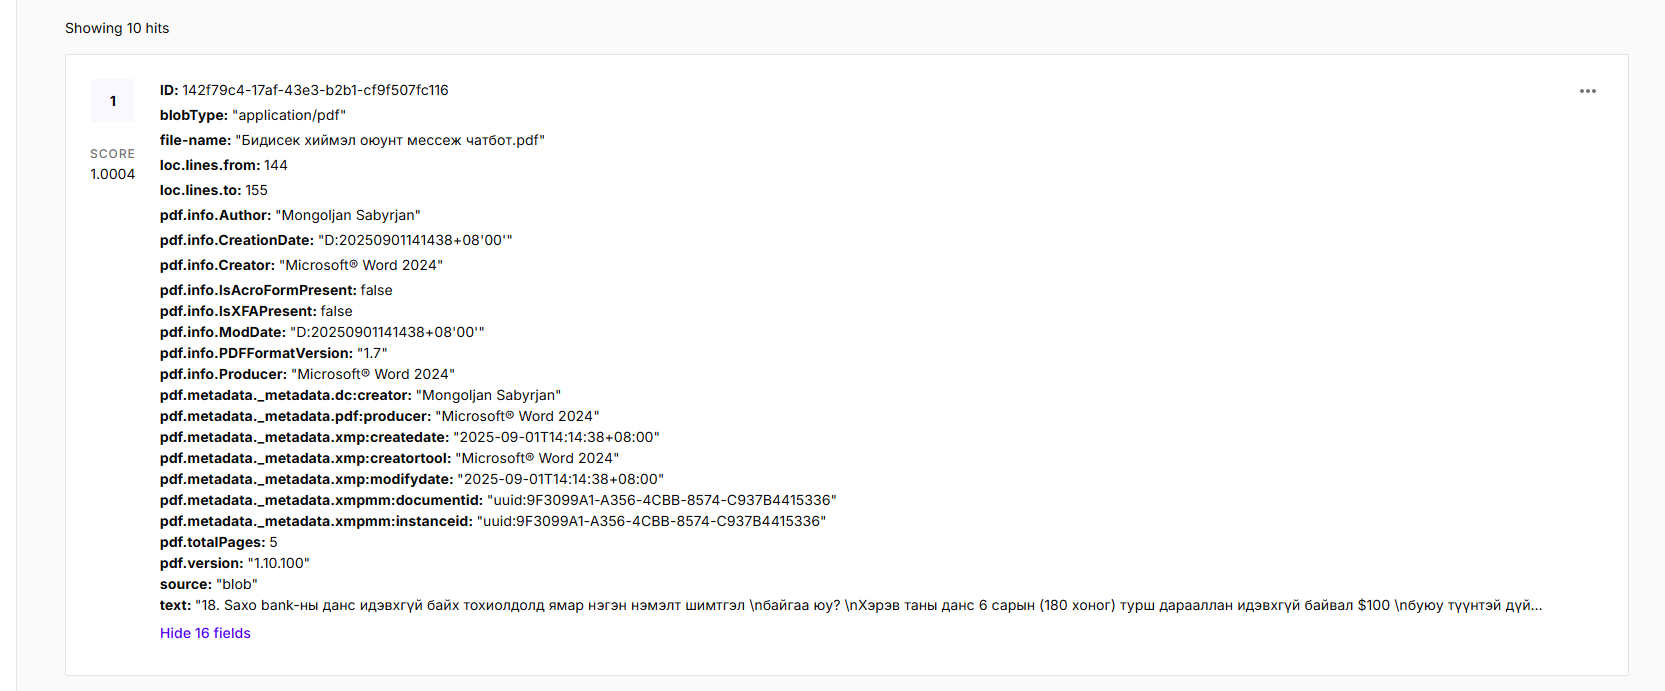
\includegraphics[scale=0.4]{assets/Screenshot 2025-09-04 163408.png}
    \caption{Pinecone вектор мэдээллийн сан 1 чанк}
    \label{fig:pinecone_chunk}
\end{figure}
Бичлэг доторх агуулагдаж буй текст нь харагдаж байна.
\begin{figure}[H]
    \centering
    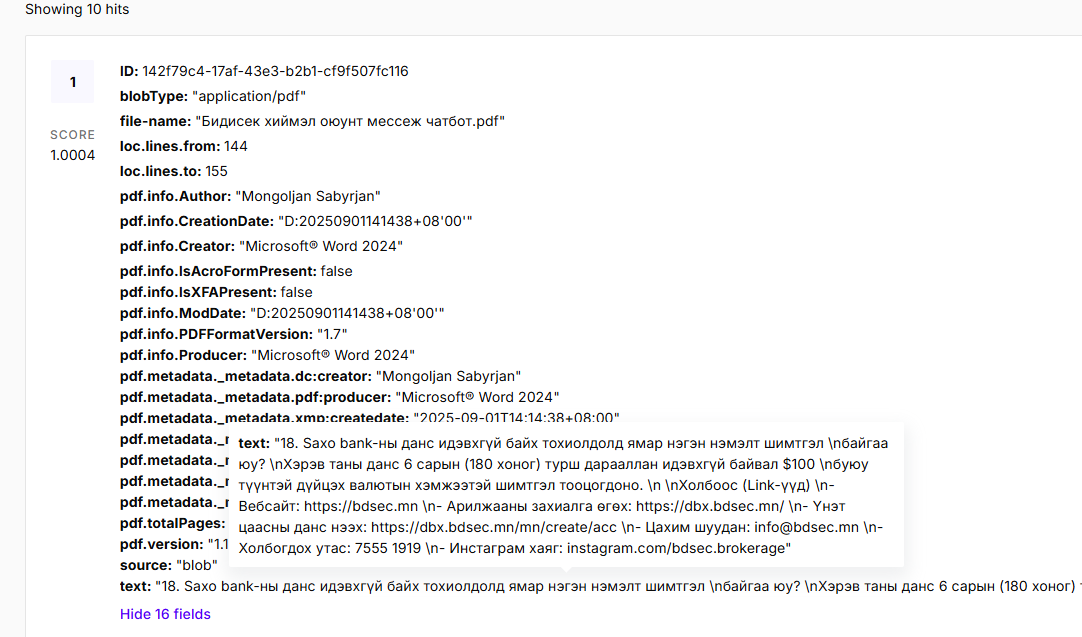
\includegraphics[scale=0.5]{assets/Screenshot 2025-09-04 163413.png}
    \caption{Pinecone вектор мэдээллийн сан дахь 1 чанкс}
    \label{fig:pinecone_chunk_text}
\end{figure}

Инстаграм дээрх чатанд хариулсны дараах үр дүн:
\begin{figure}[H]
    \centering
    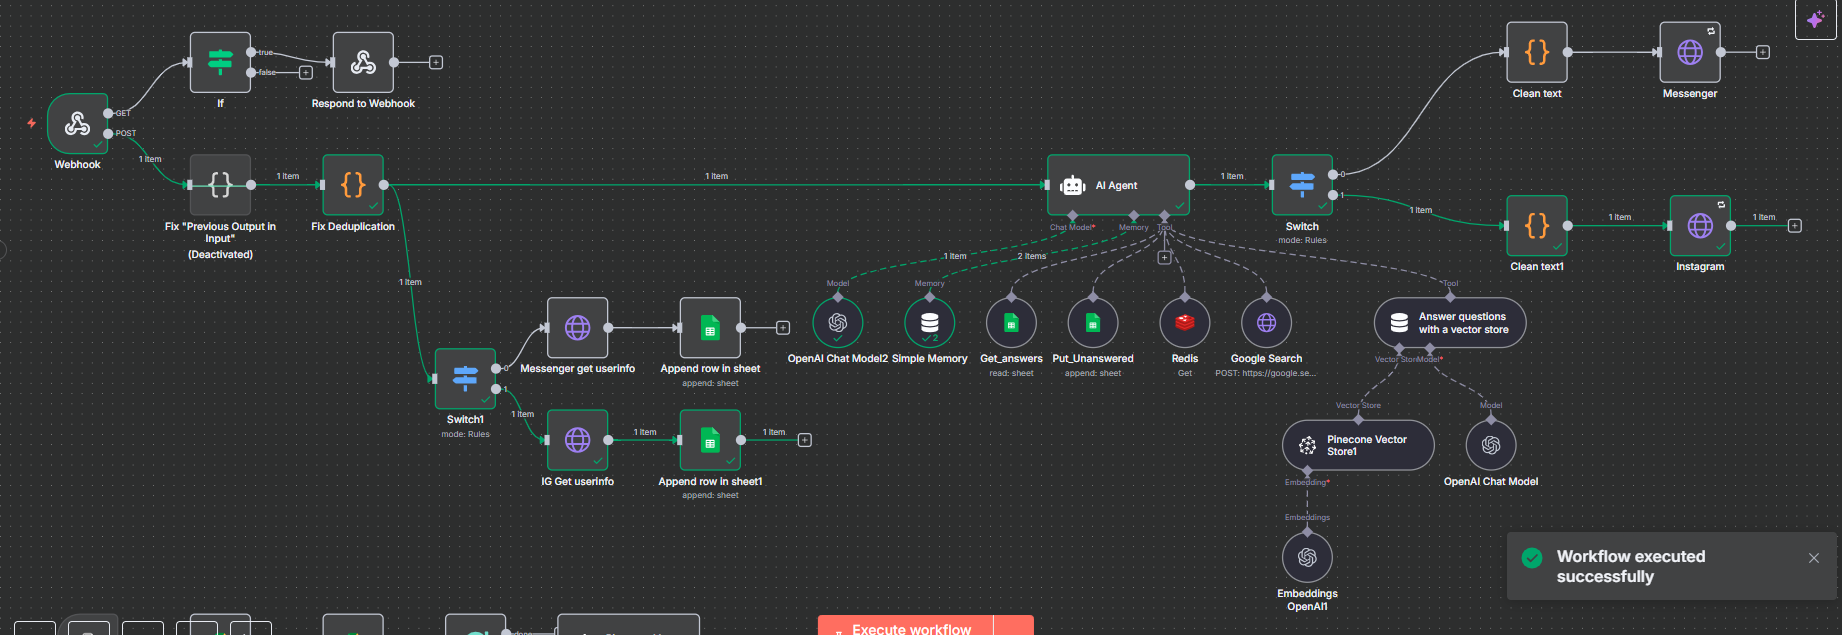
\includegraphics[scale=0.35]{assets/Screenshot 2025-09-04 163816.png}
    \caption{Инстаграм дээрх чатанд ажлын урсгал ажилласны дараа}
    \label{fig:instagram_chat_1}
\end{figure}

\begin{figure}[H]
    \centering
    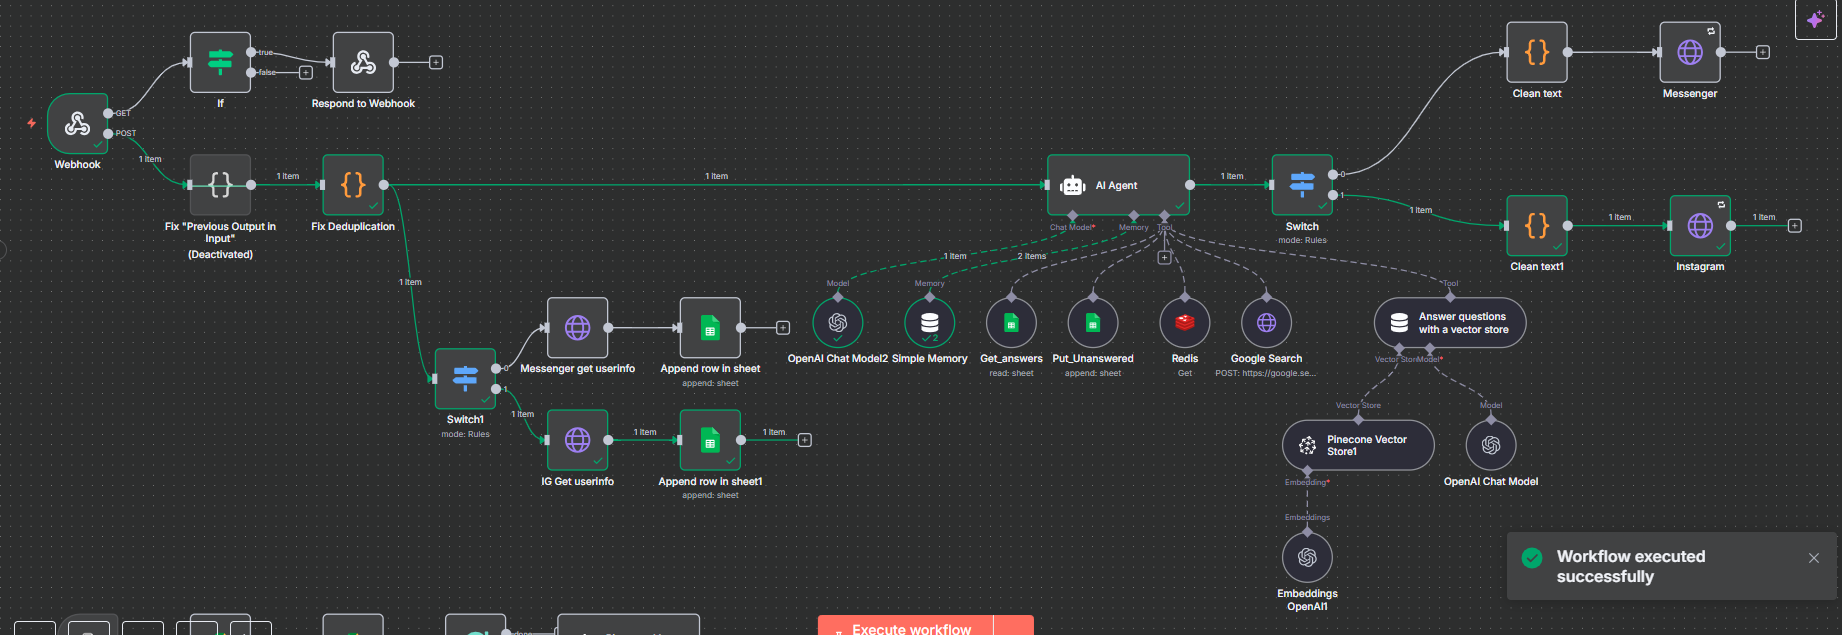
\includegraphics[scale=0.35]{assets/Screenshot 2025-09-04 163816.png}
    \caption{Инстаграм дээрх чатанд ажлын урсгал ажилласны дараа}
    \label{fig:instagram_chat_2}
\end{figure}
Хариулт
\begin{figure}[H]
    \centering
    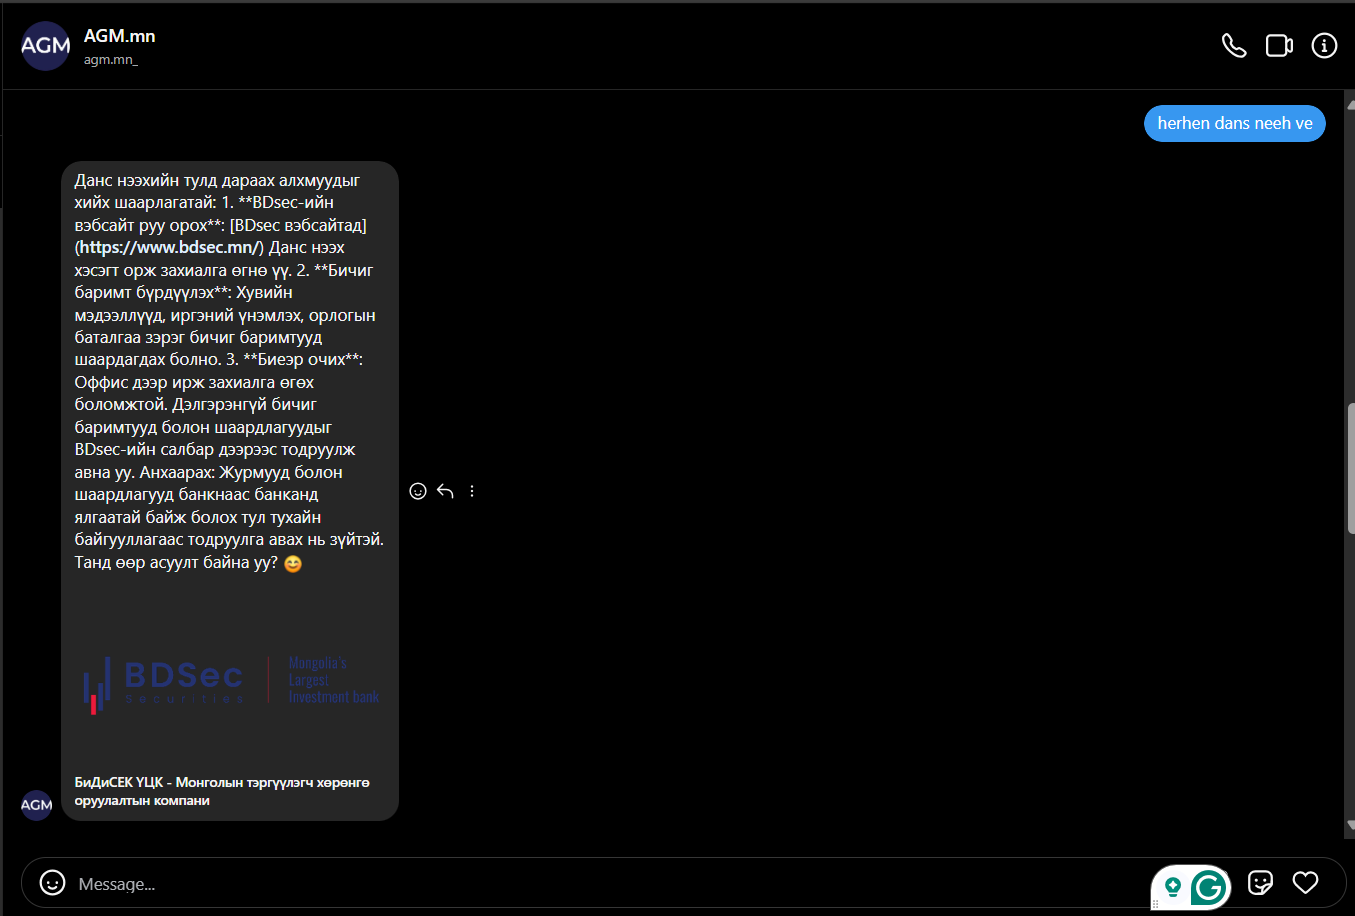
\includegraphics[scale=0.35]{assets/Screenshot 2025-09-04 214533.png}
    \caption{Инстаграм дээрх чат дээрх үр дүн}
    \label{fig:instagram_result}
\end{figure}



\begin{figure}[H]
    \centering
    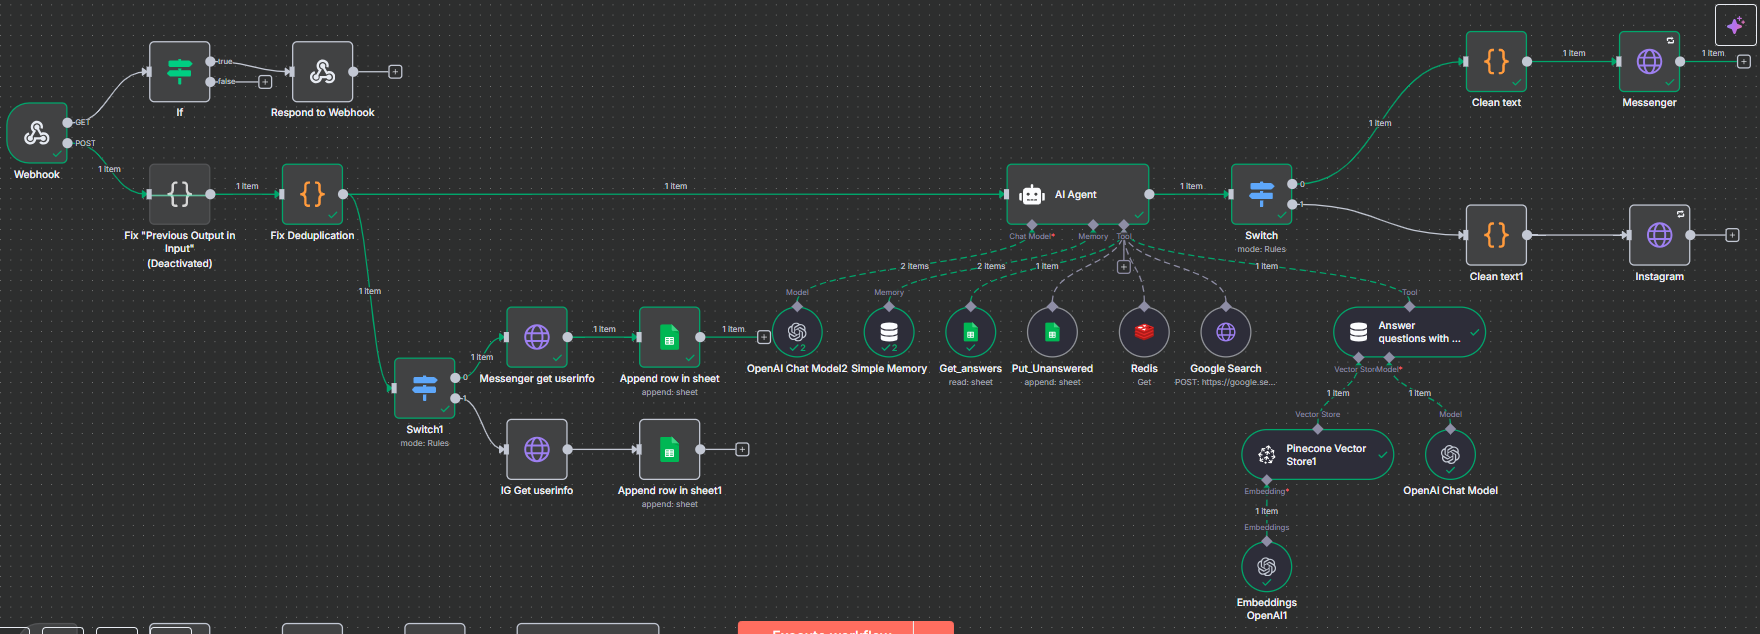
\includegraphics[scale=0.35]{assets/Screenshot 2025-09-04 163137.png}
    \caption{фейсбүүк дээрх чатанд ажлын урсгал ажилласны дараа}
    \label{fig:facebook_chat_1}
\end{figure}

Хариулт:
\begin{figure}[H]
    \centering
    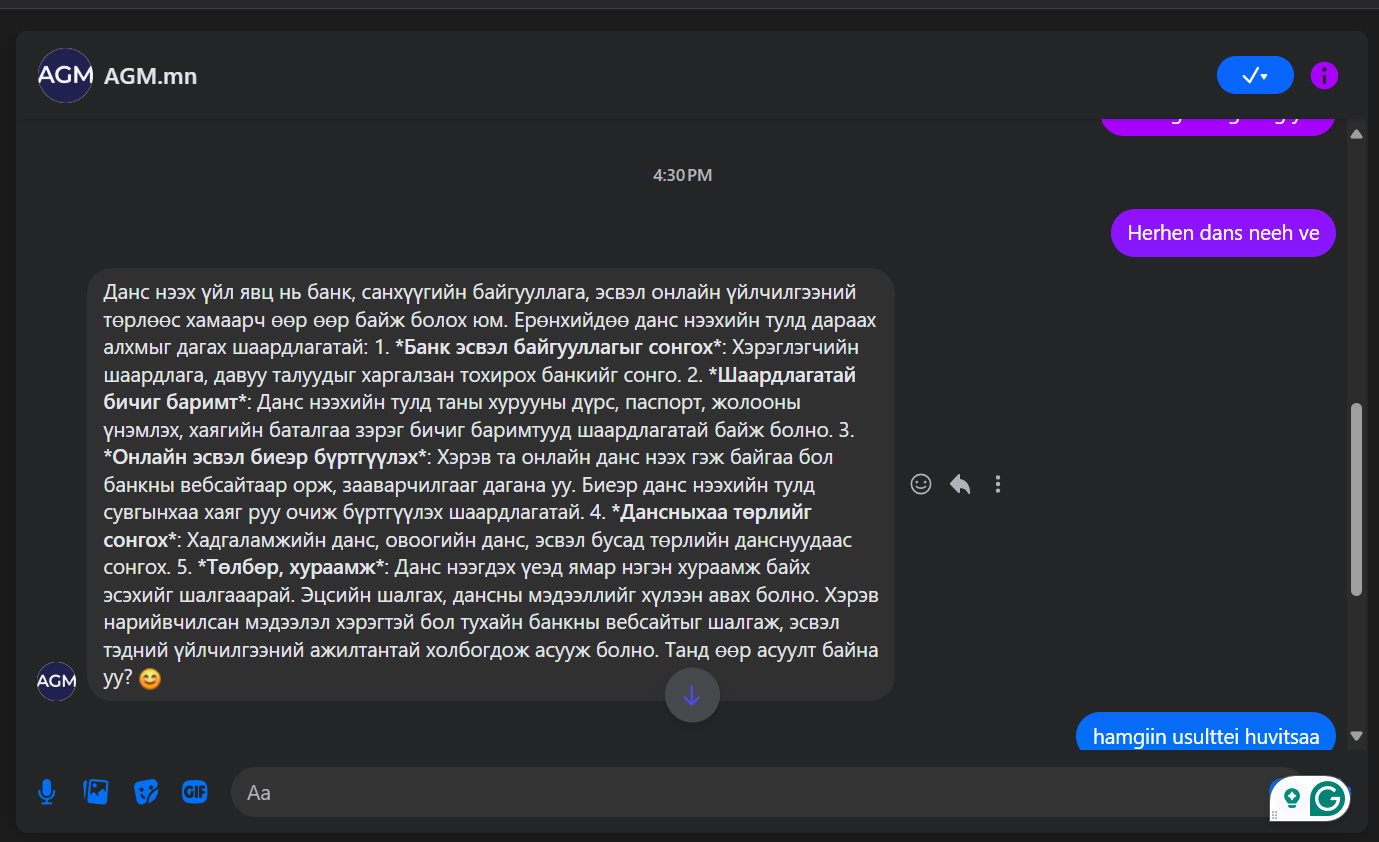
\includegraphics[scale=0.4]{assets/Screenshot 2025-09-04 214633.png}
    \caption{Фейсбүүк дээрх чат дээрх үр дүн}
    \label{fig:facebook_result_1}
\end{figure}

Хэрэглэгчээс өсөлттэй, бууралттай хувьцааны мэдээлэл асуусны дараа үндсэн ажлын урсгал ажилласан.

\begin{figure}[H]
    \centering
    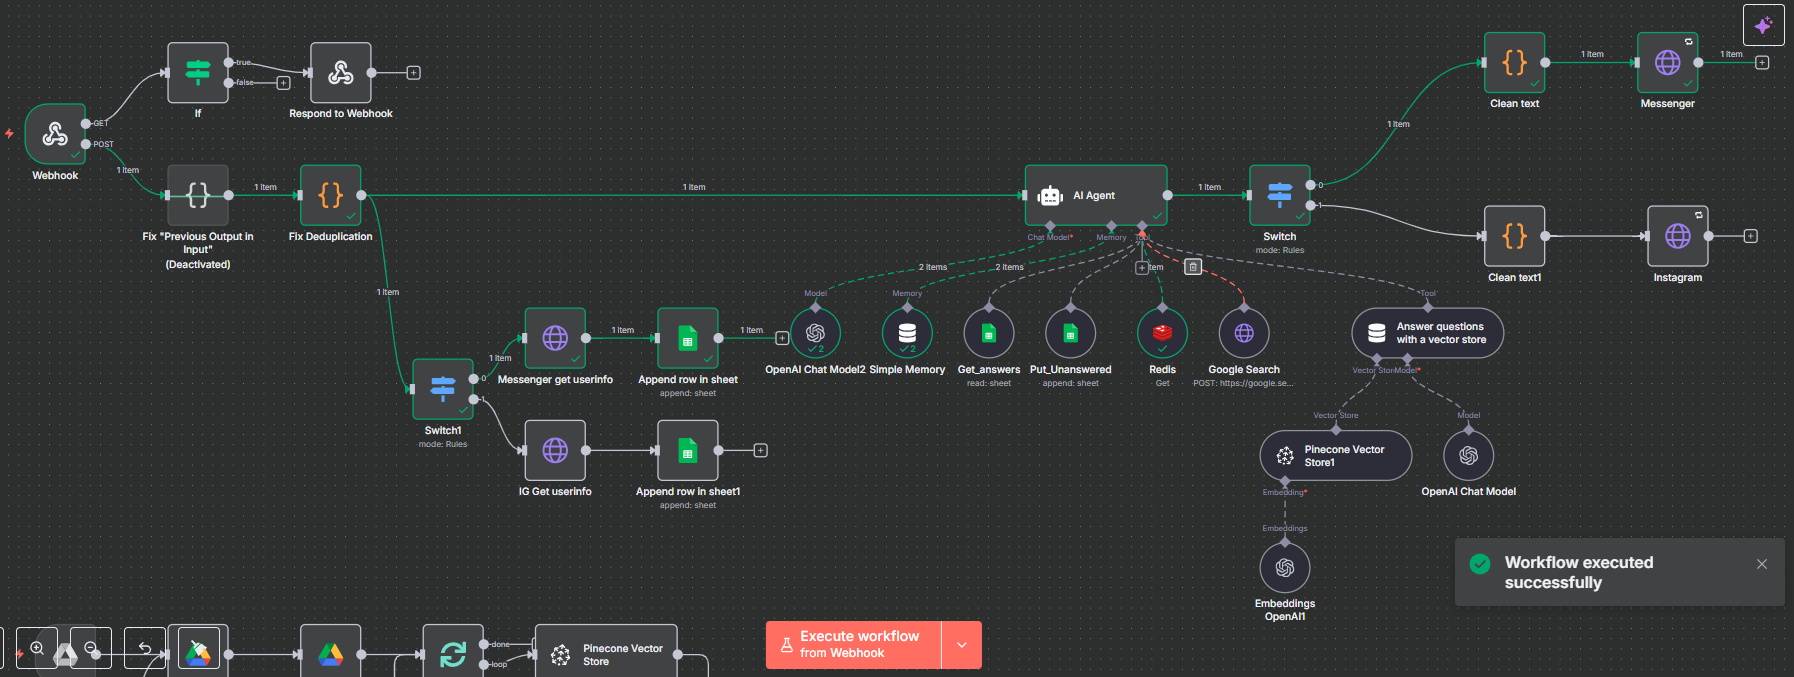
\includegraphics[scale=0.35]{assets/Screenshot 2025-09-04 163224.png}
    \caption{Фейсбүүк дээрх чат дээрх үр дүн}
    \label{fig:facebook_chat_2}
\end{figure}

\textbf{Үр дүн:}
\begin{figure}[H]
    \centering
    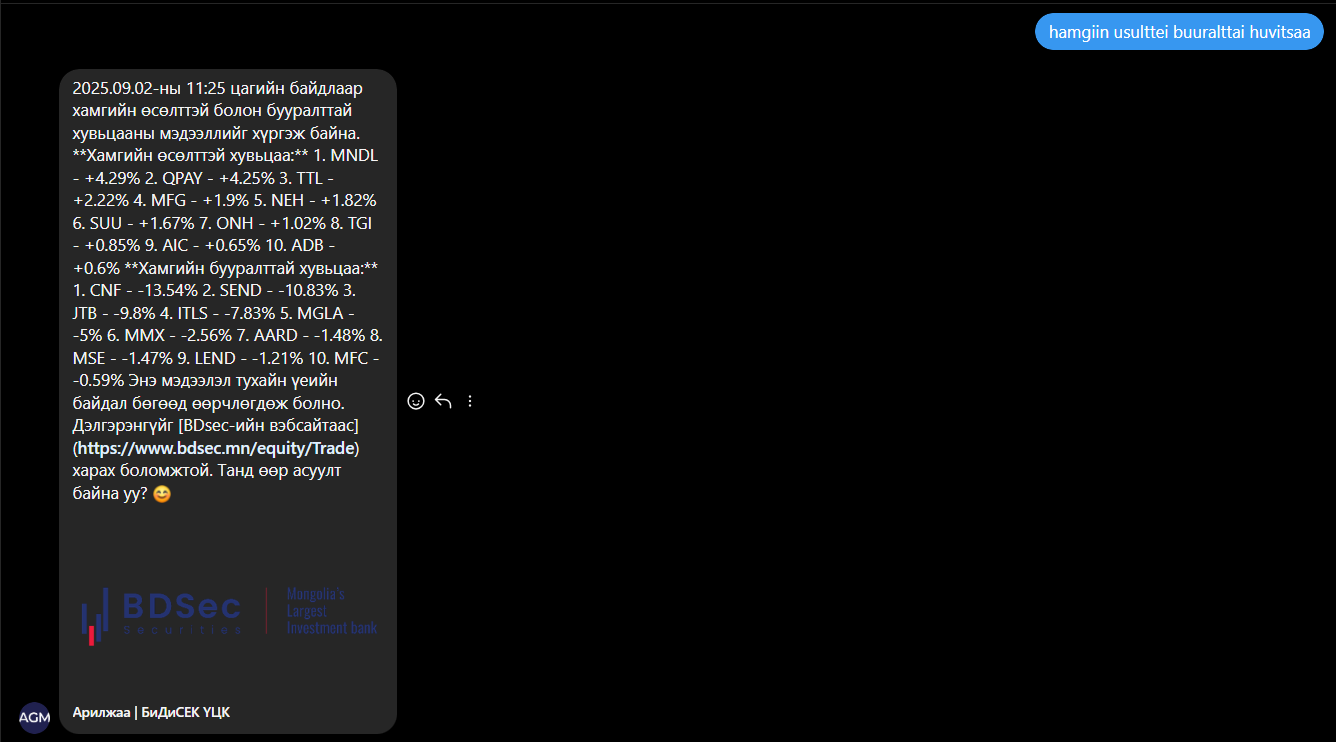
\includegraphics[scale=0.45]{assets/Screenshot 2025-09-04 214240.png}
    \caption{Чат дээрх дээрх үр дүн}
    \label{fig:facebook_result_2}
\end{figure}


\begin{figure}[H]
    \centering
    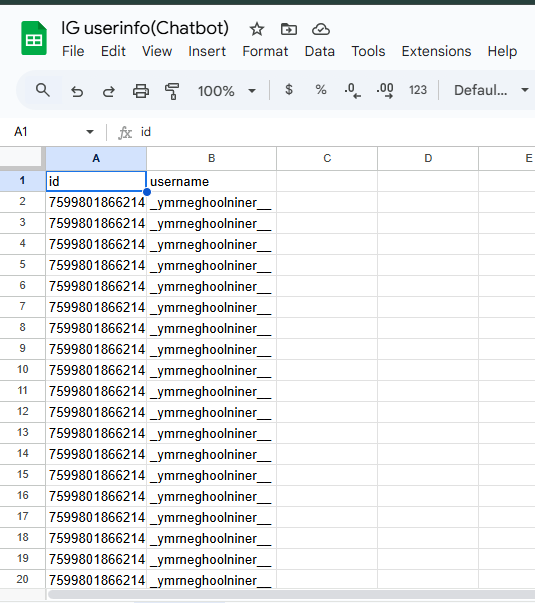
\includegraphics[scale=0.6]{assets/Screenshot 2025-09-04 155233.png}
    \caption{Google sheet дээрх хадгалсан инстаграм хаяг}
    \label{fig:google_sheet_instagram}
\end{figure}


\begin{figure}[H]
    \centering
    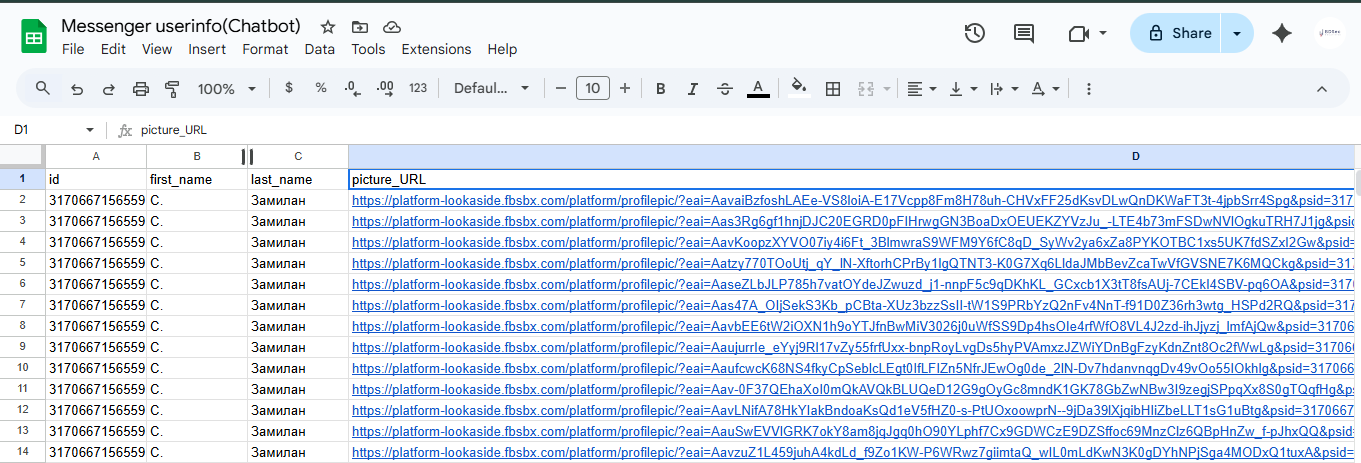
\includegraphics[scale=0.45]{assets/Screenshot 2025-09-04 155201.png}
    \caption{Google sheet дээрх хадгалсан фейсбүүк хаяг}
    \label{fig:google_sheet_facebook}
\end{figure}

\begin{figure}[H]
    \centering
    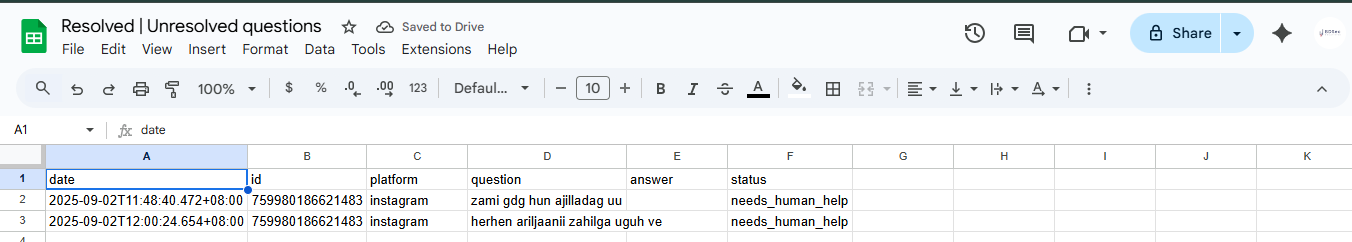
\includegraphics[scale=0.45]{assets/Screenshot 2025-09-04 155216.png}
    \caption{Google sheet дээрх хадгалсан хариулж чадаагүй асуултууд}
    \label{fig:google_sheet_unanswered}
\end{figure}